\pagebreak
%\thispagestyle{empty}
%\flushleft
\textbf{\large Supplemental Materials: NCBI's Virus Discovery Hackathon: Engaging Research Communities to Identify Cloud Infrastructure Requirements}
\setcounter{equation}{0}
\setcounter{figure}{0}
\setcounter{table}{0}
%\setcounter{page}{0}
\setcounter{section}{0}
\renewcommand{\theequation}{S\arabic{equation}}
\renewcommand{\thefigure}{S\arabic{figure}}
\renewcommand{\bibnumfmt}[1]{[S#1]}
\renewcommand{\citenumfont}[1]{S#1
\renewcommand{\thefigure}{S\arabic{figure}}}
\renewcommand{\thepart}{\arabic{part}}
\renewcommand\thesection{Supplementary Material~\arabic{section}}
\renewcommand\thesubsection{\alph{subsection})}
\renewcommand\thesubsubsection{\roman{subsection})}

\section{Dark Matter Methods}
  \label{sec:sm_dm}
  Contigs designated as 'known\_unknonw' were analyzed for potential novel
  viruses. The contigs were screened for open reading frames (ORFs) and hidden
  Markov Models (HMMs) using VIGA \cite{Gonzalez-Tortuero2018}. VIGA was
  deployed with the following virus databases: pVOG \cite{Grazziotin2017}, RVDB
  \cite{Goodacre2018}, and Virus RefSeq \cite{Brister2015}. The tabular VIGA
  output was converted into a local SQLite database to facilitate its
  exploration using SQL queries and to export the results in JSON
  \cite{rfc_json} for indexing (DarkMatter1/tools/make-vigodb/src/mk-vigodb.py,
  FIG Z).

  The VIGA output was extended by calculating the virus quotient for each VIGA
  hit. The virus quotient is defined by the percentage of viral genes used to
  train the HMM amongst total genes. To better assess the predicted  VIGA
  annotations, we developed a simple scoring system for the BLASTx and DIAMOND
  results from VIGA:
  $\frac{similarity_{reported} + coverage_{reported}}{200} - evalue_{reported}$.
  A score of 1 indicates the predictions is identical to the templates used  by
  VIGA while a score of 0 indicates no templates  were found by VIGA. The VIGA
  SQLite database was queried for “eukaryotic virus” in the annotations column
  and contigs with high scores and "virus" in the description line were aligned
  against the non-redundant database using BLASTn and BLASTx \cite{Camacho2009}
  to further identify  these contigs. Contigs were annotated into a
  GenBank-ready format using VAPiD \cite{Shean2019}.

  \begin{figure}[h]
    \centering
    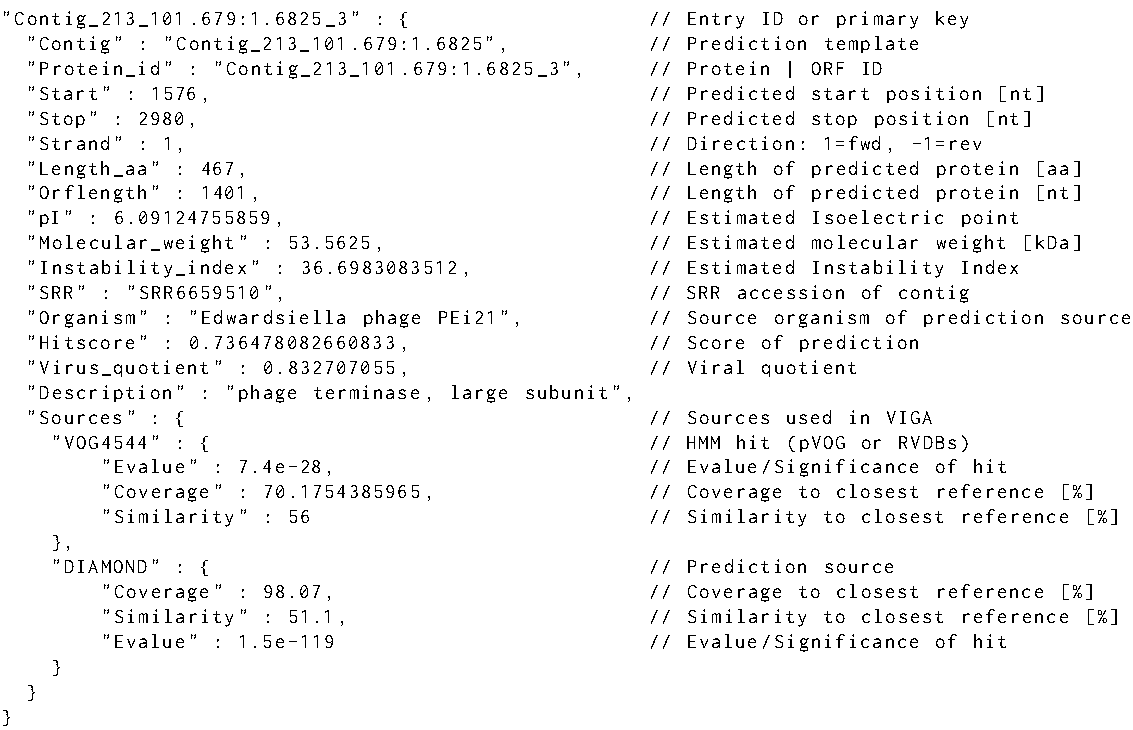
\includegraphics[width=0.6\textwidth]{figs/viga_json.pdf}
    \caption{Example of annotated  domain output in JSON format.
            \label{fig:sm_dm_outp}}
  \end{figure}

\section{Machine Learning Methods}
  \label{sec:sm_ml}
  Jaccard distance was estimated on the identified viral contigs using MASH
  \cite{Ondov2019}. MASH provides the user with a rapid method to reduce DNA sequences in
  representative k-mer sketches that are used to estimate a Jaccard similarity
  between samples. The tool was shown to be scalable in both number of
  considered metagenomes and size of the samples. MASH was shown to be a
  reliable tool to cluster amplicon datasets, metagenome read datasets and
  contig datasets \cite{Choi2018}.

  A kmer size of 21bp was chosen with a sketch size of 10,000. Samples
  containing less than two viral contigs were removed from the analysis.
  A total of 511 samples were kept for the analyzed and clustered by ward
  clustering. A manual cleaning of the terms was performed to remove
  punctuation and low-informative terms. In total, 210 samples with abstract
  and comments were analyzed.

\section{Index Methods}
  \label{sec:sm_idx}
  Setting up test data and databases: Three virtual machines were setup with
  Solr, MongoDb and PostgreSQL. Test tables were created through running a
  bigquery generate test tables with n entries to test the three databases. To
  generate these tables, we used a script saved in GitHub at:
  \url{https://github.com/NCBI-Hackathons/VirusDiscoveryProject/blob/master/ScalableIndex}.
  Three test tables were generated with 100 entries, and one million entries
  for SRA metadata, contig description and known contigs metadata. This was
  done without optimization or indexing.

  Uploading test data to the database: To upload the data to Solr, we used a
  schemaless document upload with the Solr interface. A script was used to
  import the JSON files to MongoDB (uploaded to GitHub), and another script was
  written to upload the data to PostgreSQL. PostgreSQL was the only database
  where the data types for each field needs to be defined. Overall, the data
  import for all three databases took less than a minute for the different
  databases and the test datasets generated.

  Indexing the field: Solr indexes all the fields in the document when uploaded
  as a schemless import. No fields were indexed for MongoDB and PostgreSQL with
  the current setup and files. This could have serious performance
  consequences, as the lookup complexity for non-indexed sql is usually
  considered on the order of n, where n is the number of elements in the
  database. For searching where an indexed field is used as the primary clause,
  the complexity is $n * log(n)$.











